\documentclass[]{article}
\usepackage[utf8]{inputenc}
\usepackage[spanish]{babel}
\usepackage[margin=2cm]{geometry}
\usepackage{amsmath}
\usepackage{graphicx}
\usepackage{amssymb}
\usepackage{booktabs}
\usepackage{hyperref}
\usepackage{longtable}
\usepackage{subcaption}
\usepackage{float}
\usepackage{caption}

\title{Tarea 3: Implementación computacional de cálculo de reticulados \\ [0.5em] \large ICE2006 - 1}
\author{Agustin Bustamante}


\begin{document}
	
	\maketitle
	
	\newpage
	
	\section{Introducción y Objetivos}
	Este informe presenta la resolución de problemas de estática relacionados a a sistemas de reticulado tanto en 2D como en 3D mediante el uso del lenguaje de programación Python. El método permite la resolución de sistemas de barras articuladas de forma sistemática, ensamblando las ecuaciones de equilibrio a modo de matriz y resolviéndolas como un sistema lineal. Adicionalmente se abordó el diseño de un puente de reticulado el cual debe estar sujeto a ciertas restricciones geométricas.
	\section{Marco Teórico}
	\subsection{Método matricial para reticulados 2D}
	Para el metodo matricial de reticulados, el equilibrio de fuerzas en cada nod o es expresado de manera general a traves del sistema:
	\begin{equation}
		[Bf | Lr] \cdot [\begin{bmatrix}
			S \\ R
		\end{bmatrix}]^T = -F
	\end{equation}
	donde $B_f \in \mathbb{R} \land (2n x m)$ es la matriz con los cosenos directores de los elementos, $L_r \in \mathbb{R} \land (2n x r)$es la matriz de reacciones de los nodos, $S\in \mathbb{R} \land m$ es el vector correspondiente a los esfuerzos internos de las barras, $R\in\mathbb{R} \land r$ es el vector que representa las restricciones en los apoyos y $F\in \mathbb{R} \land (2n)$ corresponde al vector e fuerzas externas aplicadas. Considerando que n es el numero de nodos, m el número de elementos y r la cantidad de grados de libertad restringidos.
	
	Para cada elemento e conectado a los nodos i y j, su longitud y cosenos directores están dados por
	\begin{equation}
		L_c = \sqrt{(x_j - x_i)^2 + (y_j - y_i)^2}
	\end{equation}
	
	\begin{equation}
		C_x = (x_j - x_i)/L_c
	\end{equation}
	 
	\begin{equation}
		c_y = (y_j - y_i)/L_c
	\end{equation}
	
	Las columnas de $B_f$ poseen los cosenos directores en las filas de su respectivo nodo asignando por convención a las filas del nodo $i$ como positivas y las del nodo $j$ como negativas. Reflejando de esta forma como actúa la fuerza interna de una barra en sus distintos extremos.
	
	La matriz $L_r$ es una matriz de ceros la cual cuenta con un 1 en la posición que corresponda a cada grupo de libertad restringido, lo que nos permite incluir las reacciones que desconocemos del sistema. Por convención los signo adoptan valor positivo en tracción y negativo en compresión.
	
	\subsection{Extensión para casos 3D}
	El uso de este método para resolución de sistemas tridimensionales es altamente similar, la particular diferencia es que se debe considerar el coseno director del eje z y la distancia al eje z para calcular el largo:
	\begin{equation}
		L_c = \sqrt{(x_j - x_i)^2 + (y_j - y_i)^2 + (z_j - z_i)^2}
	\end{equation}
	\begin{equation}
		c_z = (z_j - z_i)/L_c
	\end{equation}
	Como directa consecuencia del ajuste tridimensional es lógico deducir que las nuevas dimensiones para las matrices son para  $B_f \in \mathbb{R} \land (3n x m)$, para  $B_f \in \mathbb{R} \land (3n x r)$, para $F\in \mathbb{R} \land (2n)$ y $R$ se mantiene igual.
	
	\subsection{Diseño puente - (Problema 3)}
	\subsubsection{Selección de forma}
	
	El reticulado de la pista vehicular fue modelado como una parábola:
	\begin{equation}
		f(x) = ax^2 + bx + c
	\end{equation}
	Los parámetros para de esta función fueron determinados aplicando las siguientes restricciones:
	\begin{itemize}
		\item f(0) = 0 (inicio en el nodo (0,0))
		\item f´(67.5) = 0 (alcanzar el máximo en el nodo central)
		\item $f(50)\geq 15m $ 
	\end{itemize}
	De estas restricciones podemos se obtiene que:
	\begin{equation}
		c = 0
	\end{equation}
	\begin{equation}
		b = -135a
	\end{equation}
	\begin{equation}
		a\leq -0.00353
	\end{equation}
	
	basado en estas restricciones se eligio por conveniencia a = -0.004, lo cual determina b = 0.54 resultando:
	\begin{equation}
		f(x) = -0.004x^2 + 0.54x
	\end{equation}
	
	\subsubsection{División de tramos}
	La pista vehicular fue dividida en 18 tramos rectos, es decir 19 nodos, esto implica una separación horizontal de $\vartriangle{x} = 135/18 = 7.5 m$. Este numero fue elegido bajo los siguientes criterios:
	\begin{itemize}
		\item Todo elemento del sistema debe de medir $\leq 12 m$
		\item Un numero par de tramos implica un numero impar de nodos, por lo que se asegura la existencia de un nodo central, con el fin de mantener la simetría del reticulado
		\item Aproximación visual de que los elementos diagonales mas largos del soporte superior cumplan con la condición de ser $\leq 12m$
	\end{itemize}
	
	\subsubsection{Determinar altura del soporte superior}
	Los nodos del cordón superior se ubican de manera vertical a los nodos de la pista a una altura adicional de $a$ metros. Con el fin de maximizar la altura estructural pero manteniéndose en las restricciones de largo máximo, por geometría se puede deducir que los elementos mas largos de la estructura serán los que se conecten de forma diagonal al nodo central del puente basado en esto se puede plantear la ecuación:
	\begin{equation}
		L_{max} = \sqrt{7.5^2 + (0.225 - a)^2} \leq 12 m
	\end{equation}
	despejando la ecuación se puede ver que $a\leq 9.59 m$. De lo cual se adopto $a = 9,5 m$ por conveniencia y para seguir cumpliendo con la restricción.
	
	\subsubsection{Restricciones de resistencia}
	Cada elemento debe cumplir con ciertos limites de fuerza máxima que pueden recibir.
	Si el elemento se encuentra en tracción:
	\begin{itemize}
		\item $F_{trac} \leq 2750 kN$
	\end{itemize}
	mientras que si el elemento se encuentra en compresion debe cumplir con:
	\begin{itemize}
		\item $F_{comp} \leq 2750 kN$
		\item $F_{comp} \leq (24000\pi ^2 / L_c^2)$
	\end{itemize}
	Donde $L_c$ corresponde al largo del elemento en metros.
	El factor de seguridad de cada elemento esta dado por:
	\begin{equation}
		FS = s_{max} / s_{adm}
	\end{equation}
	
	\newpage
	
	\section{Presentación de Resultados}
	\subsection{Problema 1 b.1}
	\subsubsection{Numeración de nodos y elementos}
	\begin{figure}[!htbp]
		\centering
		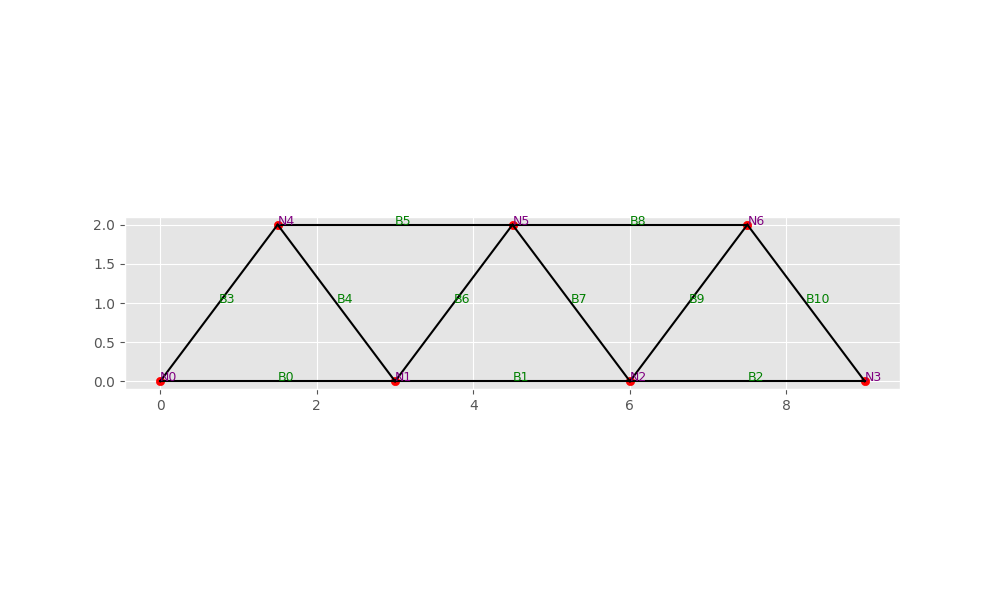
\includegraphics[width=0.6\textwidth]{Nodos_reticulado_p1.png}
		\caption{Representación Nodos}
		\label{fig:Ploteo nodos_p1_b1}
	\end{figure}
	
	\subsubsection{Resultados matrices resueltas:}
	
	\begin{table}[htbp]
		\centering
		\caption{Datos vector S}
		\label{tab: Vector_S_P1_b1}
		\begin{tabular}{lc}
			\toprule
			\textbf{Elemento} & S\textbf{(kN)} \\
			\midrule
			0 & -0.053\\
			1 & -1.982\\
			2 & -1.661\\
			3 & 10.059\\
			4 & -1.607\\
			5 & 8.812\\
			6 & 1.607\\
			7 & 3.393\\
			8 & 7.740\\
			9 & 2.857\\
			10 & 2.768\\
			\bottomrule
		\end{tabular}
	\end{table}
	
	\begin{table}[htbp]
		\centering
		\caption{Datos vector R}
		\label{tab: Vector_R_P1_b1}
		\begin{tabular}{lc}
			\toprule
			\textbf{Elemento} & S\textbf{(kN)} \\
			\midrule
			0 & -5.982\\
			0 & -8.047\\
			3 & -2.214\\
			\bottomrule
		\end{tabular}
	\end{table}
	\begin{table}[htbp]
		\centering
		\caption{Datos matriz Rid}
		\label{tab: Tabla_Rid_P1_b1}
		\begin{tabular}{lcc}
			\toprule
			\textbf{Nodo} & \textbf{$R_x$} & \textbf{$R_y$} \\
			\midrule
			0 & -5.982) & -8.047\\
			3 & 0 & -2.214 \\
			\bottomrule
		\end{tabular}
	\end{table}
	
	\begin{figure}[!htbp]
		\centering
		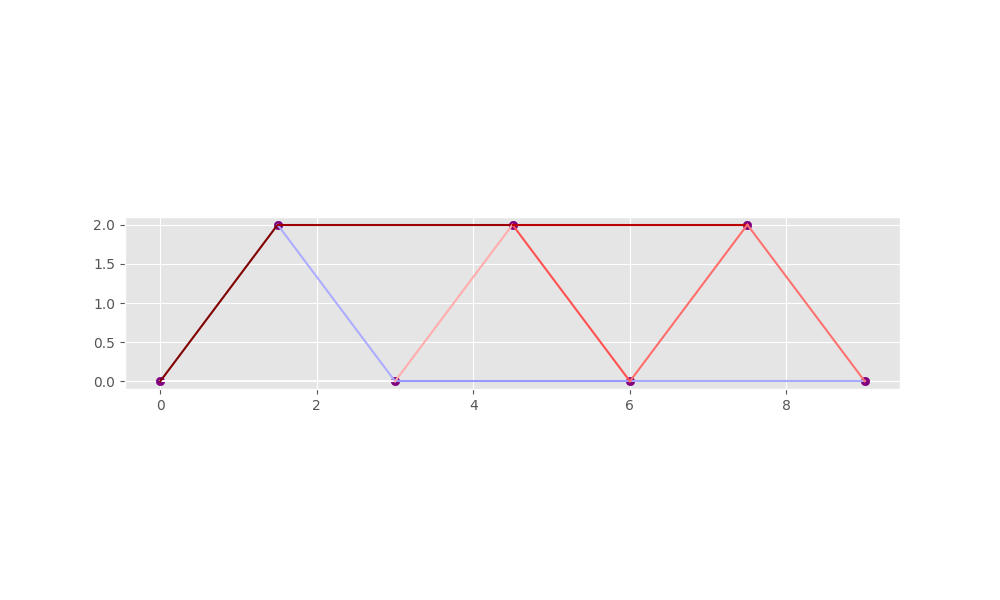
\includegraphics[width=0.6\textwidth]{Fuerzas_reticulado_p1.png}
		\caption{Representación Fuerzas}
		\label{fig:Ploteo_fuerzas_p1_b1}
	\end{figure}
	
	\newpage
	\subsection{Problema 1 b.2}
	\subsubsection{Numeración de nodos y elementos}
	\begin{figure}[!htbp]
		\centering
		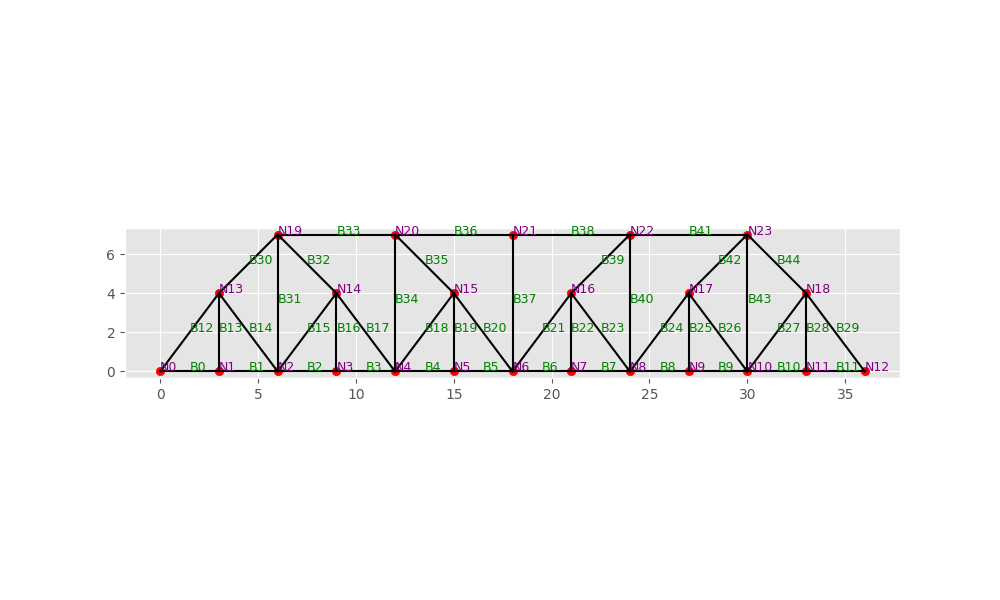
\includegraphics[width=0.6\textwidth]{Nodos_reticulado_p2.png}
		\caption{Representación Nodos}
		\label{fig:Ploteo nodos_p1_b2}
	\end{figure}
	
	\subsubsection{Resultados matrices resueltas:}
	
	\begin{table}[htbp]
		\centering
		\caption{Datos vector S}
		\label{tab: Vector_S_P1_b2}
		\begin{tabular}{lc}
			\toprule
			\textbf{Elemento} & S\textbf{(kN)} \\
			\midrule
			0 & -709.092\\
			1 & -709.092\\
			2 & -735.395\\
			3 & -735.395\\
			4 & -975.567\\
			5 & -975.567\\
			6 & -992.048\\
			7 & -992.048\\
			8 & -604.324\\
			9 & -604.324\\
			10 & -446.689\\
			11 & -446.689\\
			12 & 512.113  \\
			13 & 100         \\
			14 & -144.588\\
			15 & 49.250 \\
			16 & 0.          \\
			17 & -344.752\\
			18 & 55.534 \\
			19 & -75.        \\
			20 & -13.735\\
			21 & 13.735 \\
			22 & -250        \\
			23 & 176.609\\
			24 & -469.598\\
			25 & 0.          \\
			26 & 67.085 \\
			27 & -195.640\\
			28 & -125.       \\
			29 & 744.482\\
			30 & 557.229\\
			31 & -43.730\\
			32 & -334.322\\
			33 & 728.041\\
			34 & 231.375\\
			35 & -58.776\\
			36 & 932.299\\
			37 & 0      \\
			38 & 932.299\\
			39 & -138.203\\
			40 & 234.390\\
			41 & 717.432\\
			42 & -455.391\\
			43 & 102.844 \\
			44 & 444.167\\
			\bottomrule
		\end{tabular}
	\end{table}
	
	\begin{table}[htbp]
		\centering
		\caption{Datos vector R}
		\label{tab: Vector_R_P1_b2}
		\begin{tabular}{lc}
			\toprule
			\textbf{Elemento} & S\textbf{(kN)} \\
			\midrule
			0 & 401.825\\
			0 & -409.690\\
			12 & -595.585\\
			\bottomrule
		\end{tabular}
	\end{table}
	\begin{table}[htbp]
		\centering
		\caption{Datos matriz Rid}
		\label{tab: Tabla_Rid_P1_b2}
		\begin{tabular}{lcc}
			\toprule
			\textbf{Nodo} & \textbf{$R_x$} & \textbf{$R_y$} \\
			\midrule
			0 & 401.825 & -409.690\\
			12 & 0 & -595.585 \\
			\bottomrule
		\end{tabular}
	\end{table}
	
	\begin{figure}[!htbp]
		\centering
		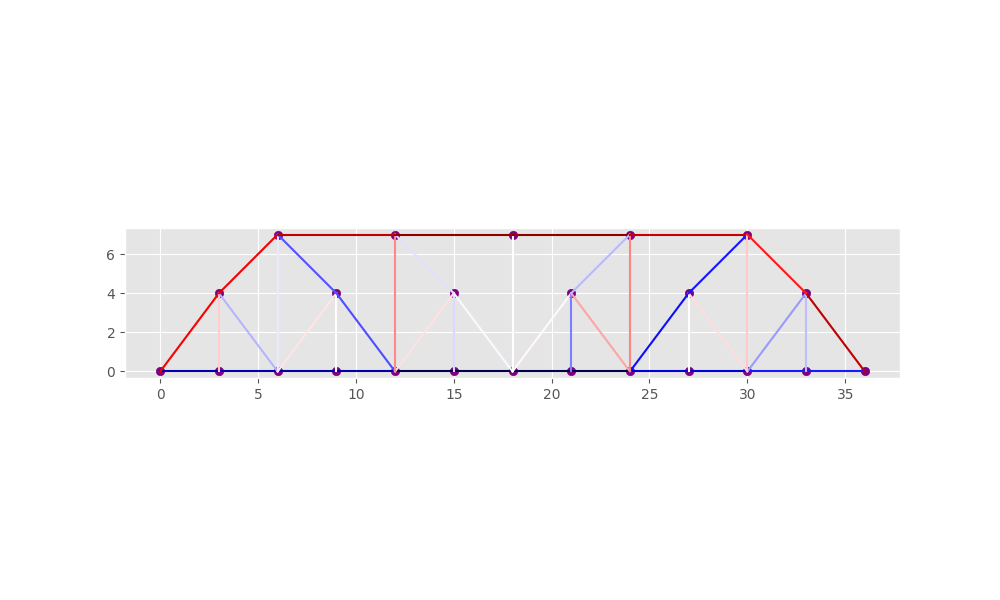
\includegraphics[width=0.6\textwidth]{Fuerzas_reticulado_p2.png}
		\caption{Representación Fuerzas}
		\label{fig:Ploteo_fuerzas_p1_b2}
	\end{figure}
	
	\newpage
	
	\subsection{Problema 2 b.1}
	\subsubsection{Numeración de nodos y elementos}
	\begin{figure}[!htbp]
		\centering
		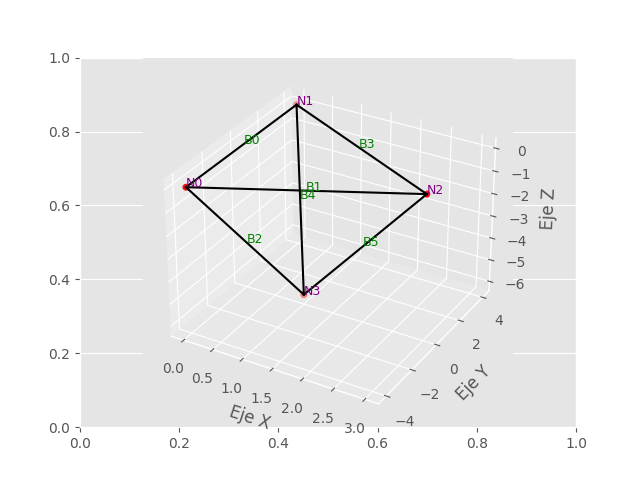
\includegraphics[width=0.6\textwidth]{Nodos_reticulado_p3.png}
		\caption{Representación Nodos}
		\label{fig:Ploteo nodos_p2_b1}
	\end{figure}
	
	\subsubsection{Resultados matrices resueltas:}
	
	\begin{table}[htbp]
		\centering
		\caption{Datos vector S}
		\label{tab: Vector_S_P2_b1}
		\begin{tabular}{lc}
			\toprule
			\textbf{Elemento} & S\textbf{(kN)} \\
			\midrule
			0 & 14.815\\
			1 & 9.259\\
			2 & -40.445\\
			3 & 9.259\\
			4 & -40.445\\
			5 & -35.136\\
			\bottomrule
		\end{tabular}
	\end{table}
	
	\begin{table}[htbp]
		\centering
		\caption{Datos vector R}
		\label{tab: Vector_R_P2_b1}
		\begin{tabular}{lc}
			\toprule
			\textbf{Elemento} & S\textbf{(kN)} \\
			\midrule
			0 & -8.882\\
			0 & -33.333\\
			1 & 1.776\\
			1 & 0\\
			1 & -33.333\\
			2 & -33.333\\
			\bottomrule
		\end{tabular}
	\end{table}
	\begin{table}[htbp]
		\centering
		\caption{Datos matriz Rid}
		\label{tab: Tabla_Rid_P2_b1}
		\begin{tabular}{lccc}
			\toprule
			\textbf{Nodo} & \textbf{$R_x$} & \textbf{$R_y$} & \textbf{$R_z$} \\
			\midrule
			0 & -8.882 & 0 & -33.333\\
			1 & 1.776 & 0 & -33.333\\
			2 & 0 & 0 & -33.333\\
			\bottomrule
		\end{tabular}
	\end{table}
	
	\begin{figure}[!htbp]
		\centering
		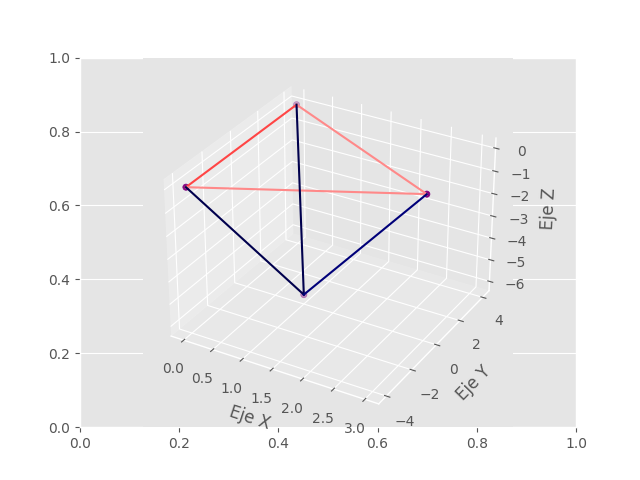
\includegraphics[width=0.6\textwidth]{Fuerzas_reticulado_p3.png}
		\caption{Representación Fuerzas}
		\label{fig:Ploteo_fuerzas_p2_b1}
	\end{figure}
	
	\newpage
	
	\subsection{Problema 2 b.2}
	\subsubsection{Numeración de nodos y elementos}
	\begin{figure}[!htbp]
		\centering
		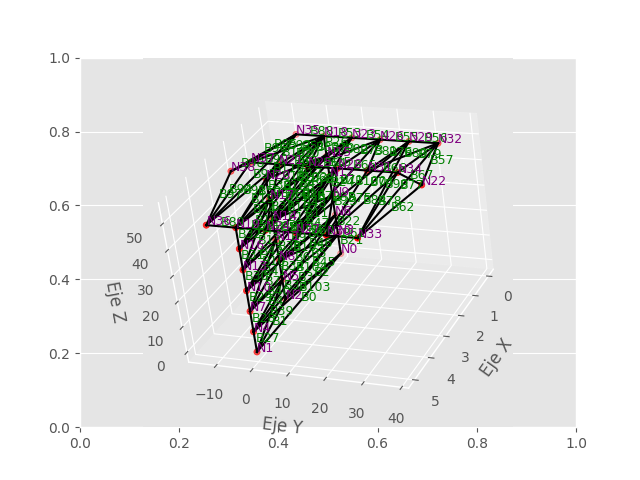
\includegraphics[width=0.6\textwidth]{Nodos_reticulado_p4.png}
		\caption{Representación Nodos}
		\label{fig:Ploteo nodos_p2_b2}
	\end{figure}
	
	\subsubsection{Resultados matrices resueltas:}
	
	\begin{longtable}{lc}
		\caption{Datos vector S}
		\label{tab:Vector_S_P2_b2} \\
		\toprule
		\textbf{Elemento} & S\textbf{(kN)} \\
		\midrule
		\endfirsthead
		
		\multicolumn{2}{c}%
		{{\bfseries Continuación de la tabla \ref{tab:Vector_S_P2_b2}}} \\
		\toprule
		\textbf{Elemento} & S\textbf{(kN)} \\
		\midrule
		\endhead
		
		\midrule
		\multicolumn{2}{r}{{Continúa en siguiente página...}} \\
		\endfoot
		
		\endlastfoot
		0 & 2.4233807e-27  \\
		1 & -3.48388937e-11 \\
		2 & -4.20078264e-12 \\
		3 & 1.21169035e-27 \\
		4 & -0            \\
		5 & -3.44820123e-12 \\
		6 & -3.23117427e-27 \\
		7 & -1.51360908e-26 \\
		8 & -0            \\
		9 & -1.00974196e-28 \\
		10 & -0            \\
		11 & 2.66036276e-13 \\
		12 & 0             \\
		13 & -3.85034061e-13 \\
		14 & -0            \\
		15 & -2.8050572e-27 \\
		16 & -0            \\
		17 & 1.36423567e-13 \\
		18 & -3247.7254182  \\
		19 & -7343.90688021 \\
		20 & -7343.90688021 \\
		21 & 16607.27050184 \\
		22 & 16607.27050184 \\
		23 & 16607.27050184 \\
		24 & 16607.27050184 \\
		25 & 16607.27050184 \\
		26 & 16607.27050184 \\
		27 & 16607.27050184 \\
		28 & 16607.27050184 \\
		29 & 16607.27050184 \\
		30 & 16607.27050184 \\
		31 & 16607.27050184 \\
		32 & 16607.27050184 \\
		33 & 17625.45899633 \\
		34 & 17625.45899633 \\
		35 & 17625.45899633 \\
		36 & 17625.45899633 \\
		37 & 17625.45899633 \\
		38 & 17625.45899633 \\
		39 & 6.57341145e-11 \\
		40 & -6.14299252e-11 \\
		41 & 6.14299252e-11 \\
		42 & -6.09735237e-11 \\
		43 & 6.1700007e-11  \\
		44 & -6.1541671e-11 \\
		45 & 7.45666223e-11 \\
		46 & -6.80605474e-11 \\
		47 & 6.80605474e-11 \\
		48 & -6.85625053e-11 \\
		49 & 6.80262463e-11 \\
		50 & -6.82836506e-11 \\
		51 & -9547.12362301 \\
		52 & 17991.20971032 \\
		53 & 30550         \\
		54 & 30550        \\
		55 & 14256.66666667 \\
		56 & 14256.66666667 \\
		57 & 6925.4154007  \\
		58 & 38696.66666667 \\
		59 & 22403.33333333 \\
		60 & 22403.33333333 \\
		61 & 6110          \\
		62 & 6925.4154007   \\
		63 & -69246.66666667 \\
		64 & -52953.33333333 \\
		65 & -36660        \\
		66 & -20366.66666667 \\
		67 & -14686.61219539 \\
		68 & 7.64168603e-15 \\
		69 & 3.95664092e-13 \\
		70 & 0             \\
		71 & -1.5158245e-13 \\
		72 & 0             \\
		73 & 3.94114371e-12 \\
		74 & 1.43992771e-14 \\
		75 & 2.95585778e-12 \\
		76 & 0           \\
		77 & -1697.22222222 \\
		78 & -2206.38888889 \\
		79 & 4412.77777778  \\
		80 & -10496.73973855 \\
		81 & 10496.73973855 \\
		82 & -10496.73973855 \\
		83 & 10496.73973855 \\
		84 & 10496.73973855 \\
		85 & -10496.73973855 \\
		86 & 10496.73973855 \\
		87 & -10496.73973855 \\
		88 & 19310        \\
		89 & 45056.66666667 \\
		90 & -64366.66666667 \\
		91 & -33173.82067945 \\
		92 & 33173.82067945 \\
		93 & -5363.88888889 \\
		94 & 13946.11111111 \\
		95 & -6973.05555556 \\
		96 & 21887.03296031 \\
		97 & 21887.03296031 \\
		98 & -46415.46341947 \\
		99 & 1.53304241e-12 \\
		100 & -1.56021091e-12 \\
		101 & 1.57067463e-12 \\
		102 & -1.58509293e-12 \\
		103 & 4.80589205e-11 \\
		104 & -4.80589205e-11 \\
		105 & 4.80589205e-11 \\
		106 & -4.80589205e-11 \\
		107 & 4.80589205e-11 \\
		108 & -4.80589205e-11 \\
		109 & 1.64818792e-12 \\
		110 & 21736.03470809 \\
	
	\end{longtable}
	
	\begin{table}[htbp]
		\centering
		\caption{Datos vector R}
		\label{tab: Vector_R_P2_b2}
		\begin{tabular}{lc}
			\toprule
			\textbf{Elemento} & S\textbf{(kN)} \\
			\midrule
			0 & -2.337\\
			0 & -3.638\\
			0 & -16607.271\\
			1 & -16607.271\\
			2 & 3.155e-11\\
			2 & -17625.459\\
			\bottomrule
		\end{tabular}
	\end{table}
	\begin{table}[htbp]
		\centering
		\caption{Datos matriz Rid}
		\label{tab: Tabla_Rid_P2_b2}
		\begin{tabular}{lccc}
			\toprule
			\textbf{Nodo} & \textbf{$R_x$} & \textbf{$R_y$} & \textbf{$R_z$} \\
			\midrule
			0 & -2.337 & -3.638 & -16607.271\\
			1 & 0 & 0 & -16607.271\\
			2 & 3.155e-11 & 0 & -17625.459\\
			\bottomrule
		\end{tabular}
	\end{table}
	
	\newpage
	
	\begin{figure}[!htbp]
		\centering
		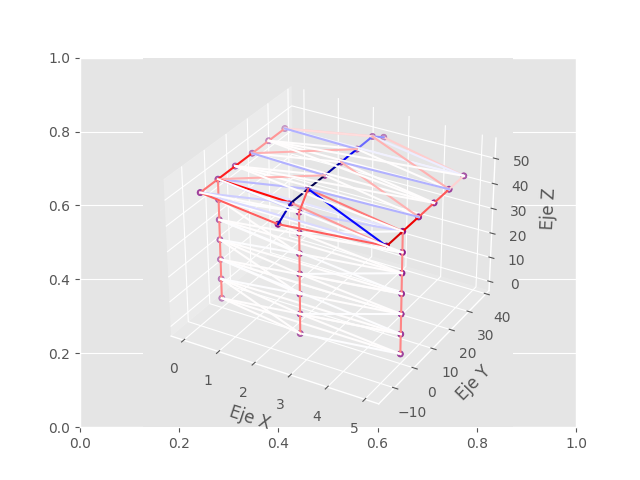
\includegraphics[width=0.6\textwidth]{Fuerzas_reticulado_p4.png}
		\caption{Representación Fuerzas}
		\label{fig:Ploteo_fuerzas_p2_b2}
	\end{figure}
	
	\subsection{Problema 3}
	\subsubsection{Numeración de nodos y elementos}
	\begin{figure}[!htbp]
		\centering
		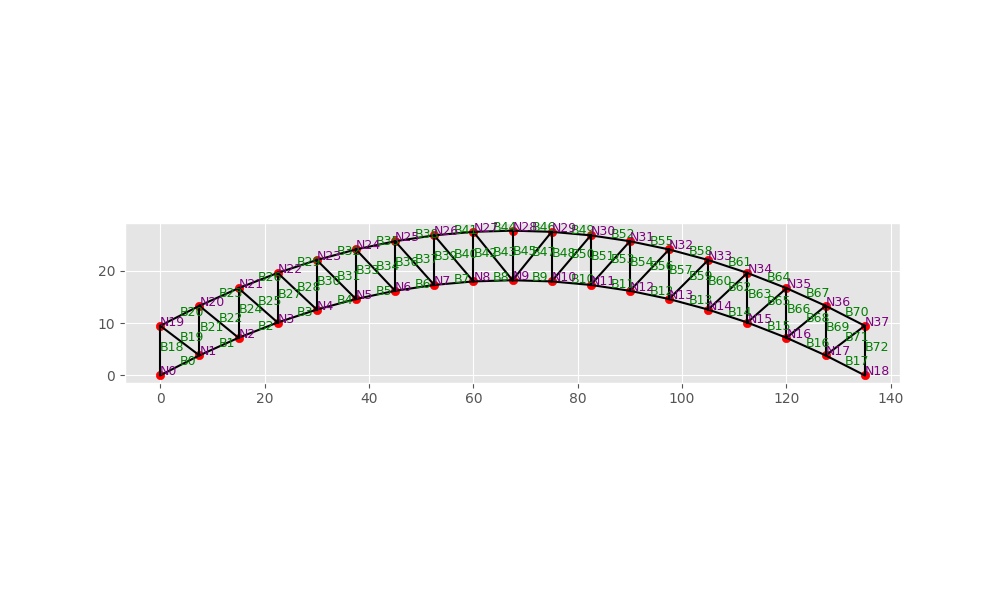
\includegraphics[width=0.6\textwidth]{Nodos_reticulado_p5.png}
		\caption{Representación Nodos}
		\label{fig:Ploteo nodos_p3}
	\end{figure}
	
	\begin{longtable}{lcccccc}
		\caption{Datos vector Tabla Problema 3}
		\label{tab:Vector_S_P3} \\
		\toprule
		\textbf{Elemento} & $C_{max}$ & $C_{adm}$& $T_{max}$& $T_{adm}$& $FS_C$& $FS_T$ \\
		\midrule
		\endfirsthead
		
		\multicolumn{7}{c}%
		{{\bfseries Continuación de la tabla \ref{tab:Vector_S_P3}}} \\
		\toprule
		\textbf{Elemento} & $C_{max}$ & $C_{adm}$& $T_{max}$& $T_{adm}$& $FS_C$& $FS_T$ \\
		\midrule
		\endhead
		
		\midrule
		\multicolumn{7}{r}{{Continúa en siguiente página...}} \\
		\endfoot
		
		\endlastfoot
		0 & 0.0 & 2750 & 0.0 & 2750 & 0.0 & 0.0                  \\
		1 & 0.0 & 2750 & 196.231 & 2750 & 0.0 & 0.071            \\
		2 & 0.0 & 2750 & 361.553 & 2750 & 0.0 & 0.131            \\
		3 & 0.0 & 2750 & 498.81 & 2750 & 0.0 & 0.181             \\
		4 & 0.0 & 2750 & 610.582 & 2750 & 0.0 & 0.222            \\
		5 & 0.0 & 2750 & 699.135 & 2750 & 0.0 & 0.254            \\
		6 & 0.0 & 2750 & 766.374 & 2750 & 0.0 & 0.279            \\
		7 & 0.0 & 2750 & 813.802 & 2750 & 0.0 & 0.296            \\
		8 & 0.0 & 2750 & 842.484 & 2750 & 0.0 & 0.306            \\
		9 & 0.0 & 2750 & 842.484 & 2750 & 0.0 & 0.306            \\
		10 & 0.0 & 2750 & 813.802 & 2750 & 0.0 & 0.296           \\
		11 & 0.0 & 2750 & 766.374 & 2750 & 0.0 & 0.279           \\
		12 & 0.0 & 2750 & 699.135 & 2750 & 0.0 & 0.254           \\
		13 & 0.0 & 2750 & 610.582 & 2750 & 0.0 & 0.222           \\
		14 & 0.0 & 2750 & 498.81 & 2750 & 0.0 & 0.181            \\
		15 & 0.0 & 2750 & 361.553 & 2750 & 0.0 & 0.131           \\
		16 & 0.0 & 2750 & 196.231 & 2750 & 0.0 & 0.071           \\
		17 & 0.0 & 2750 & 0.0 & 2750 & 0.0 & 0.0                 \\
		18 & 226.667 & 2624.604 & 0.0 & 2750 & 0.086 & 0.0       \\
		19 & 0.0 & 2677.846 & 224.402 & 2750 & 0.0 & 0.082       \\
		20 & 200.876 & 2750 & 0.0 & 2750 & 0.073 & 0.0           \\
		21 & 203.228 & 2624.604 & 24.07 & 2750 & 0.077 & 0.009   \\
		22 & 13.591 & 2526.198 & 217.449 & 2750 & 0.005 & 0.079  \\
		23 & 369.376 & 2750 & 0.0 & 2750 & 0.134 & 0.0           \\
		24 & 181.053 & 2624.604 & 46.877 & 2750 & 0.069 & 0.017  \\
		25 & 27.997 & 2381.072 & 209.979 & 2750 & 0.012 & 0.076  \\
		26 & 508.433 & 2750 & 0.0 & 2750 & 0.185 & 0.0           \\
		27 & 160.14 & 2624.604 & 68.421 & 2750 & 0.061 & 0.025   \\
		28 & 43.268 & 2243.079 & 201.919 & 2750 & 0.019 & 0.073  \\
		29 & 620.741 & 2750 & 0.0 & 2750 & 0.226 & 0.0           \\
		30 & 140.491 & 2624.604 & 88.702 & 2750 & 0.054 & 0.032  \\
		31 & 59.447 & 2112.546 & 193.202 & 2750 & 0.028 & 0.07   \\
		32 & 708.711 & 2750 & 0.0 & 2750 & 0.258 & 0.0           \\
		33 & 122.105 & 2624.604 & 107.719 & 2750 & 0.047 & 0.039 \\
		34 & 76.57 & 1989.578 & 183.769 & 2750 & 0.038 & 0.067   \\
		35 & 774.426 & 2750 & 0.0 & 2750 & 0.282 & 0.0           \\
		36 & 104.982 & 2624.604 & 125.474 & 2750 & 0.04 & 0.046  \\
		37 & 94.672 & 1874.115 & 173.566 & 2750 & 0.051 & 0.063  \\
		38 & 819.594 & 2750 & 0.0 & 2750 & 0.298 & 0.0           \\
		39 & 89.123 & 2624.604 & 141.965 & 2750 & 0.034 & 0.052  \\
		40 & 113.783 & 1765.969 & 162.547 & 2750 & 0.064 & 0.059 \\
		41 & 845.509 & 2750 & 0.0 & 2750 & 0.307 & 0.0           \\
		42 & 74.526 & 2624.604 & 157.193 & 2750 & 0.028 & 0.057  \\
		43 & 133.928 & 1664.871 & 150.669 & 2750 & 0.08 & 0.055  \\
		44 & 853.015 & 2750 & 0.0 & 2750 & 0.31 & 0.0            \\
		45 & 0.0 & 2624.604 & 51.158 & 2750 & 0.0 & 0.019        \\
		46 & 853.015 & 2750 & 0.0 & 2750 & 0.31 & 0.0            \\
		47 & 133.928 & 1664.871 & 150.669 & 2750 & 0.08 & 0.055  \\
		48 & 74.526 & 2624.604 & 157.193 & 2750 & 0.028 & 0.057  \\
		49 & 845.509 & 2750 & 0.0 & 2750 & 0.307 & 0.0           \\
		50 & 113.783 & 1765.969 & 162.547 & 2750 & 0.064 & 0.059 \\
		51 & 89.123 & 2624.604 & 141.965 & 2750 & 0.034 & 0.052  \\
		52 & 819.594 & 2750 & 0.0 & 2750 & 0.298 & 0.0           \\
		53 & 94.672 & 1874.115 & 173.566 & 2750 & 0.051 & 0.063  \\
		54 & 104.982 & 2624.604 & 125.474 & 2750 & 0.04 & 0.046  \\
		55 & 774.426 & 2750 & 0.0 & 2750 & 0.282 & 0.0           \\
		56 & 76.57 & 1989.578 & 183.769 & 2750 & 0.038 & 0.067   \\
		57 & 122.105 & 2624.604 & 107.719 & 2750 & 0.047 & 0.039 \\
		58 & 708.711 & 2750 & 0.0 & 2750 & 0.258 & 0.0           \\
		59 & 59.447 & 2112.546 & 193.202 & 2750 & 0.028 & 0.07   \\
		60 & 140.491 & 2624.604 & 88.702 & 2750 & 0.054 & 0.032  \\
		61 & 620.741 & 2750 & 0.0 & 2750 & 0.226 & 0.0           \\
		62 & 43.268 & 2243.079 & 201.919 & 2750 & 0.019 & 0.073  \\
		63 & 160.14 & 2624.604 & 68.421 & 2750 & 0.061 & 0.025   \\
		64 & 508.433 & 2750 & 0.0 & 2750 & 0.185 & 0.0           \\
		65 & 27.997 & 2381.072 & 209.979 & 2750 & 0.012 & 0.076  \\
		66 & 181.053 & 2624.604 & 46.877 & 2750 & 0.069 & 0.017 \\
		67 & 369.376 & 2750 & 0.0 & 2750 & 0.134 & 0.0           \\
		68 & 13.591 & 2526.198 & 217.449 & 2750 & 0.005 & 0.079  \\
		69 & 203.228 & 2624.604 & 24.07 & 2750 & 0.077 & 0.009   \\
		70 & 200.876 & 2750 & 0.0 & 2750 & 0.073 & 0.0           \\
		71 & 0.0 & 2677.846 & 224.402 & 2750 & 0.0 & 0.082       \\
		72 & 226.667 & 2624.604 & 0.0 & 2750 & 0.086 & 0.0       \\

\end{longtable}

\captionsetup[subfigure]{font=small, labelfont=bf, skip=2pt, justification=centering}
\setlength{\intextsep}{6pt}
\setlength{\floatsep}{6pt}

\begin{figure}[H]
	\centering
	% Fila 1
	\begin{subfigure}[b]{0.48\textwidth}
		\centering
		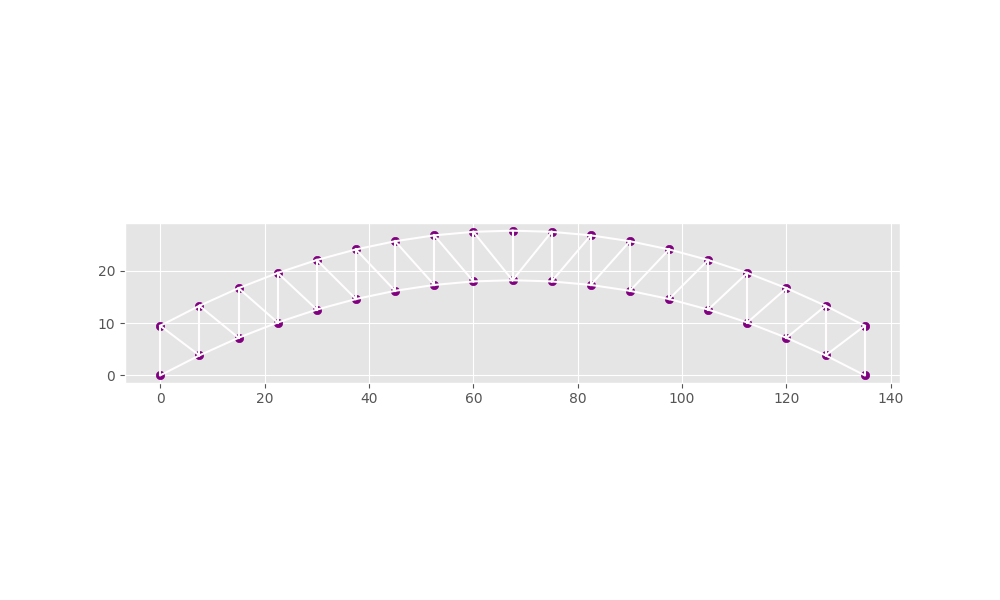
\includegraphics[width=\textwidth, trim=30 20 30 20, clip]{Fuerzas_reticulado_p5_pos1.png}
		\caption{Posición 1}
		\label{fig:p3_1}
	\end{subfigure}
	\hfill
	\begin{subfigure}[b]{0.48\textwidth}
		\centering
		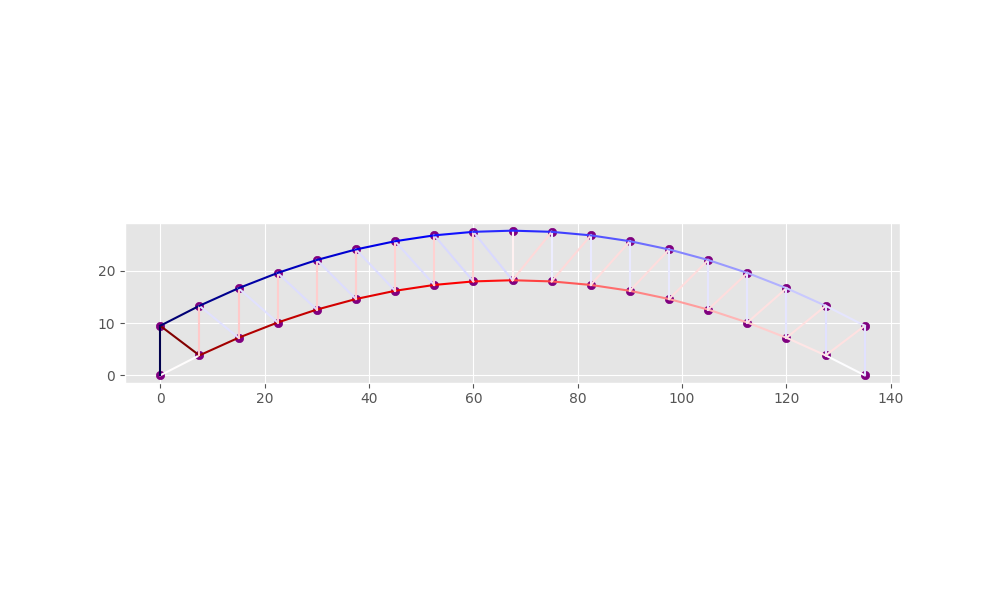
\includegraphics[width=\textwidth, trim=30 20 30 20, clip]{Fuerzas_reticulado_p5_pos2.png}
		\caption{Posición 2}
		\label{fig:p3_2}
	\end{subfigure}
	
	\vspace{3mm}
	
	% Fila 2
	
	\begin{subfigure}[b]{0.48\textwidth}
		\centering
		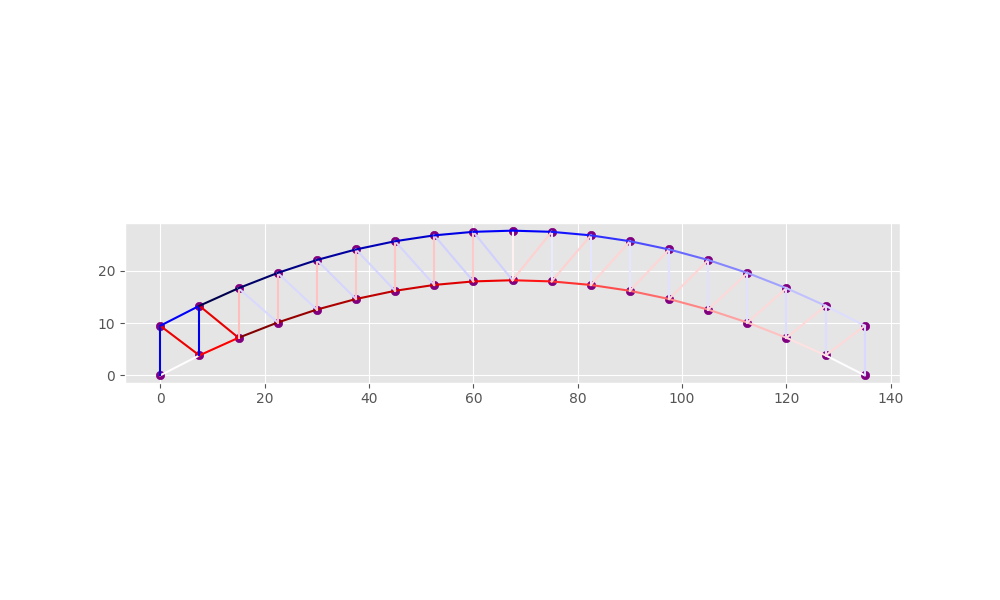
\includegraphics[width=\textwidth, trim=30 20 30 20, clip]{Fuerzas_reticulado_p5_pos3.png}
		\caption{Posición 3}
		\label{fig:p3_3}
	\end{subfigure}
	\hfill
	\begin{subfigure}[b]{0.48\textwidth}
		\centering
		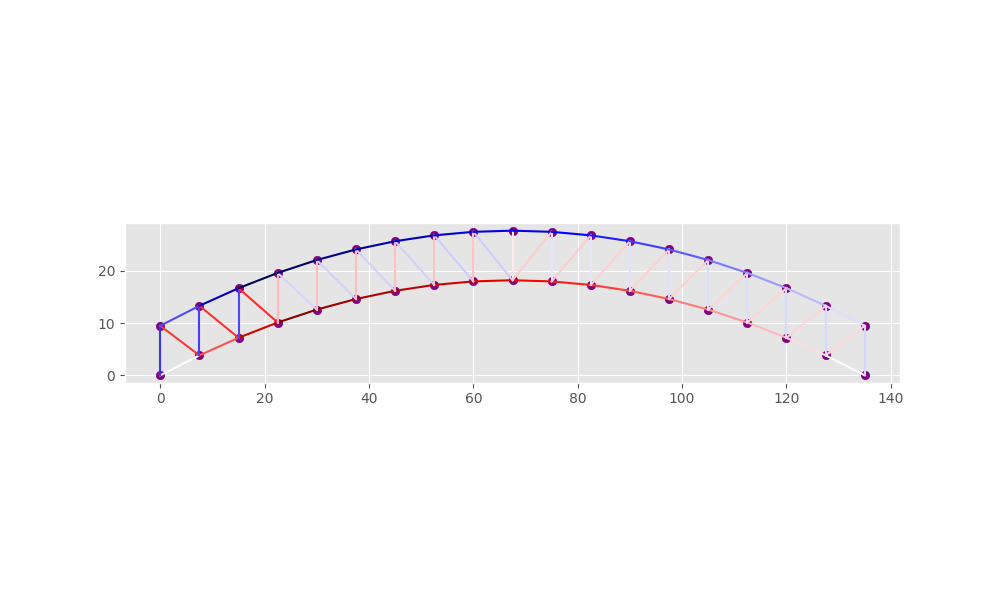
\includegraphics[width=\textwidth, trim=30 20 30 20, clip]{Fuerzas_reticulado_p5_pos4.png}
		\caption{Posición 4}
		\label{fig:p3_4}
	\end{subfigure}
	
	\caption{Diagrama de esfuerzos - carga de 240 kN para posiciones 1 a 4 (Rojo: Tracción, azul: Compresión)}
	\label{fig:esfuerzos_p3_a}
	
\end{figure}
\begin{figure}[H]\ContinuedFloat
	\centering
	
	% Fila 3
	\begin{subfigure}[b]{0.48\textwidth}
		\centering
		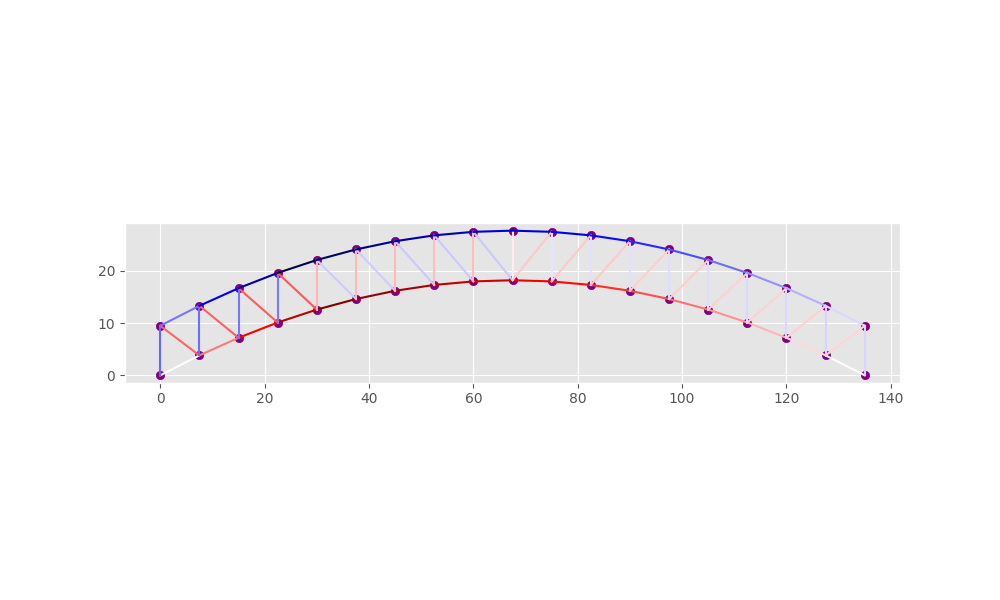
\includegraphics[width=\textwidth, trim=30 20 30 20, clip]{Fuerzas_reticulado_p5_pos5.png}
		\caption{Posición 5}
		\label{fig:p3_5}
	\end{subfigure}
	\hfill
	\begin{subfigure}[b]{0.48\textwidth}
		\centering
		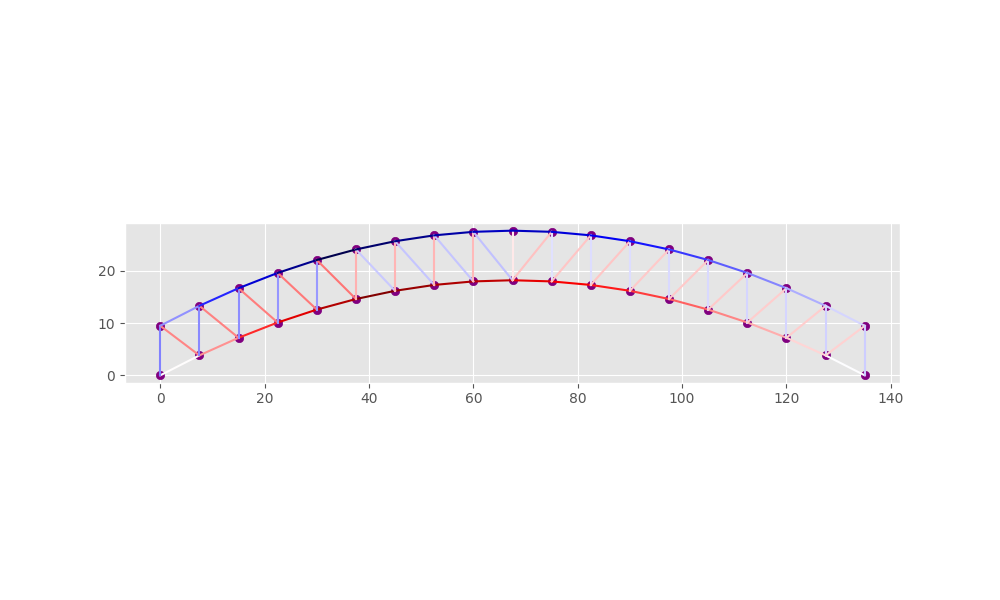
\includegraphics[width=\textwidth, trim=30 20 30 20, clip]{Fuerzas_reticulado_p5_pos6.png}
		\caption{Posición 6}
		\label{fig:p3_6}
	\end{subfigure}
	
	\vspace{3mm}
	
	% Fila 4
	\begin{subfigure}[b]{0.48\textwidth}
		\centering
		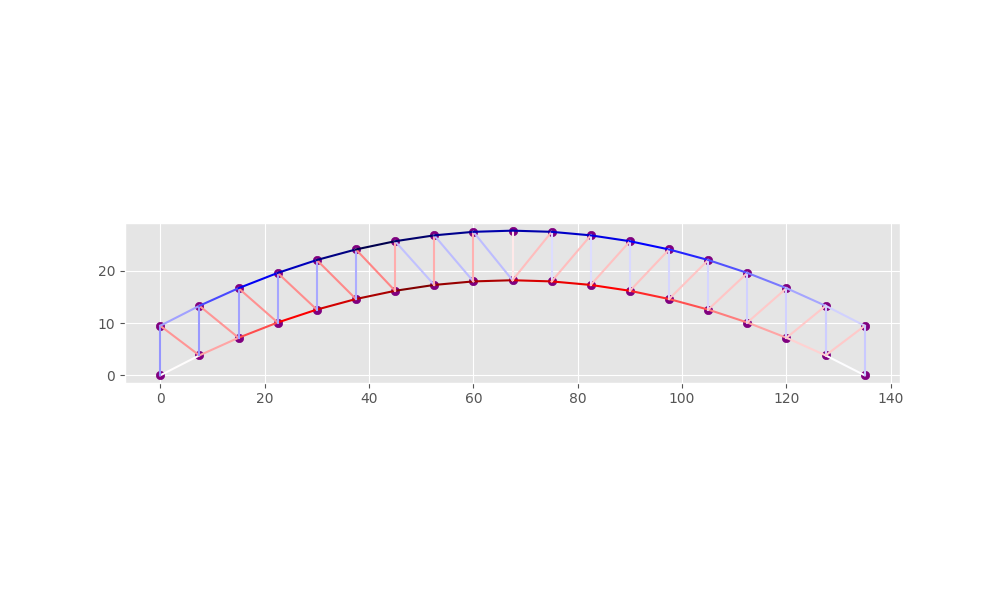
\includegraphics[width=\textwidth, trim=30 20 30 20, clip]{Fuerzas_reticulado_p5_pos7.png}
		\caption{Posición 7}
		\label{fig:p3_7}
	\end{subfigure}
	\hfill
	\begin{subfigure}[b]{0.48\textwidth}
		\centering
		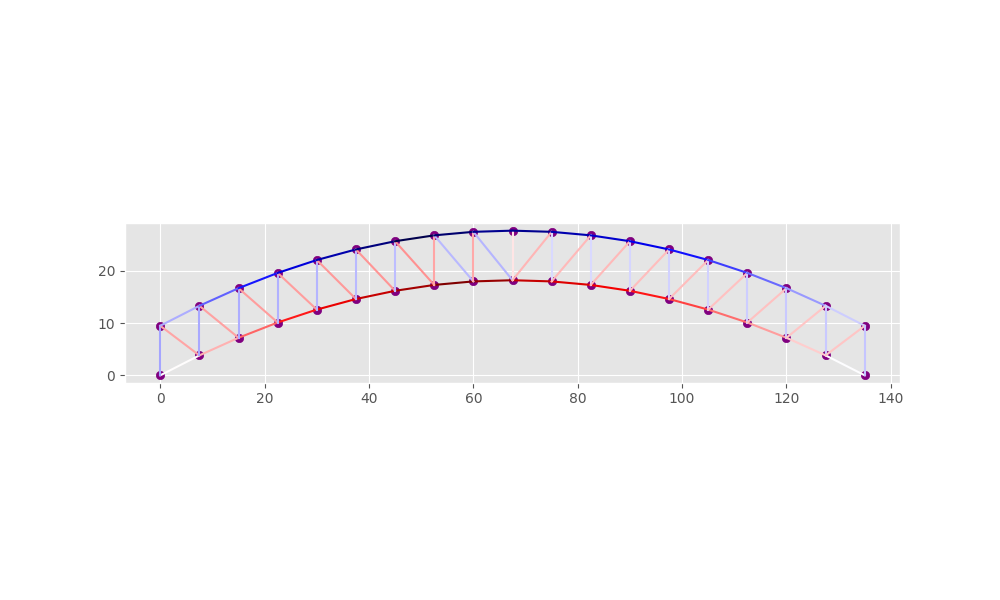
\includegraphics[width=\textwidth, trim=30 20 30 20, clip]{Fuerzas_reticulado_p5_pos8.png}
		\caption{Posición 8}
		\label{fig:p3_8}
	\end{subfigure}
	
	\caption{Diagrama de esfuerzos - carga de 240 kN para posiciones 5 a 8}
	\label{fig:esfuerzos_p3_b}
	
\end{figure}
\begin{figure}[H]\ContinuedFloat
	\centering
	
	% Fila 5
	\begin{subfigure}[b]{0.48\textwidth}
		\centering
		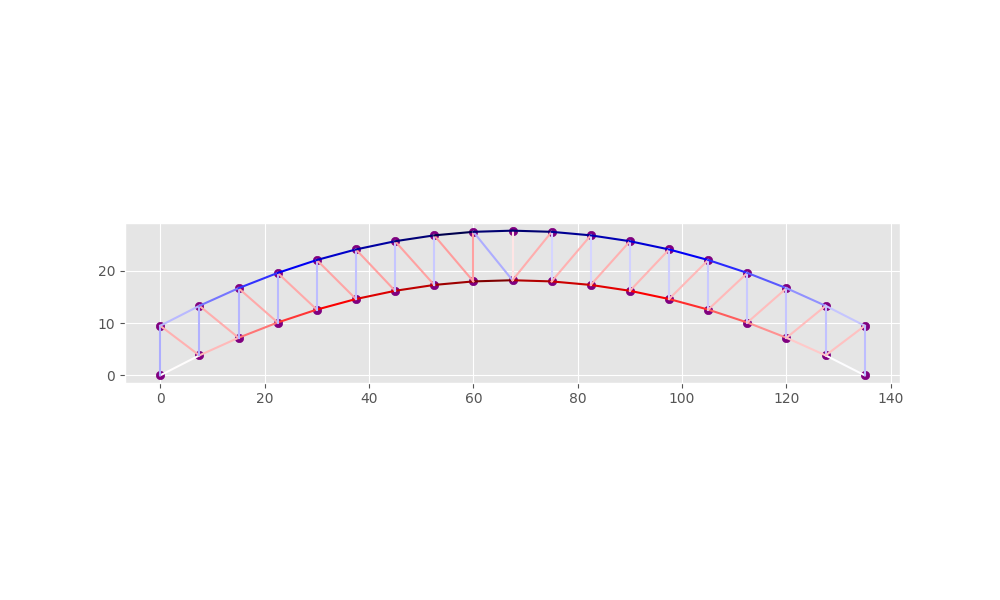
\includegraphics[width=\textwidth, trim=30 20 30 20, clip]{Fuerzas_reticulado_p5_pos9.png}
		\caption{Posición 9}
		\label{fig:p3_9}
	\end{subfigure}
	\hfill
	\begin{subfigure}[b]{0.48\textwidth}
		\centering
		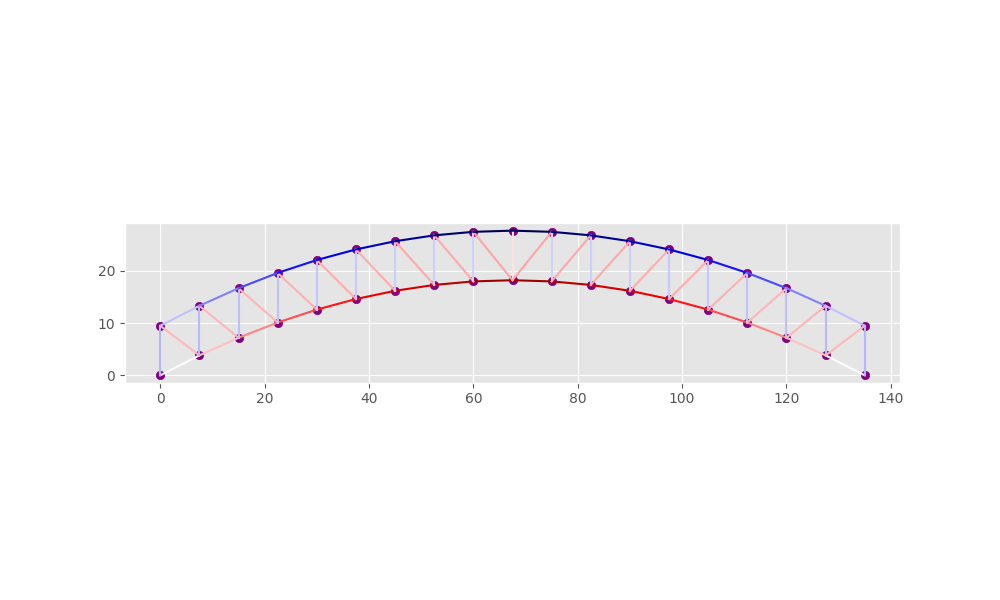
\includegraphics[width=\textwidth, trim=30 20 30 20, clip]{Fuerzas_reticulado_p5_pos10.png}
		\caption{Posición 10}
		\label{fig:p3_10}
	\end{subfigure}
	
	\vspace{3mm}
	
	% Fila 6
	\begin{subfigure}[b]{0.48\textwidth}
		\centering
		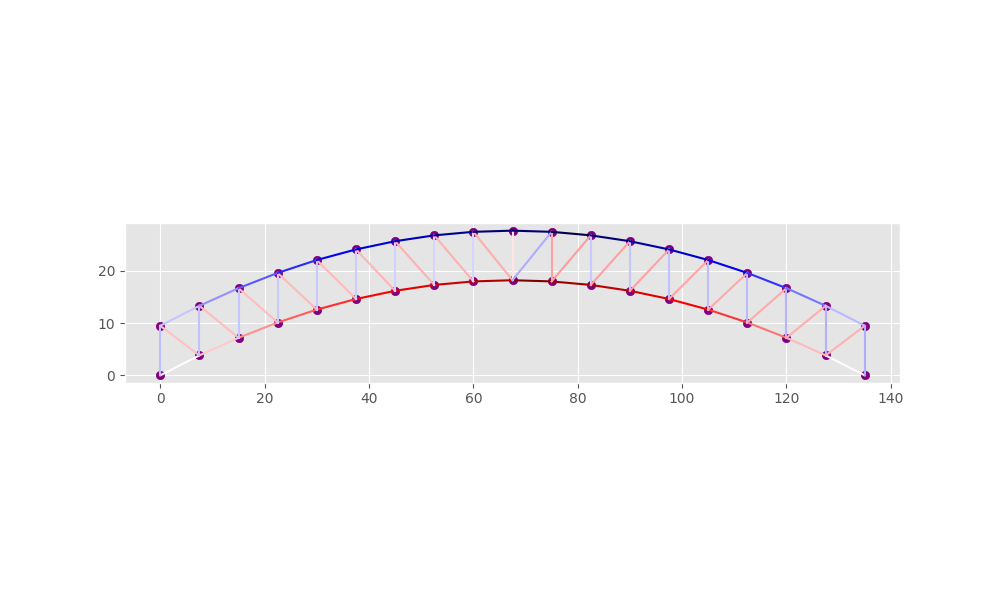
\includegraphics[width=\textwidth, trim=30 20 30 20, clip]{Fuerzas_reticulado_p5_pos11.png}
		\caption{Posición 11}
		\label{fig:p3_11}
	\end{subfigure}
	\hfill
	\begin{subfigure}[b]{0.48\textwidth}
		\centering
		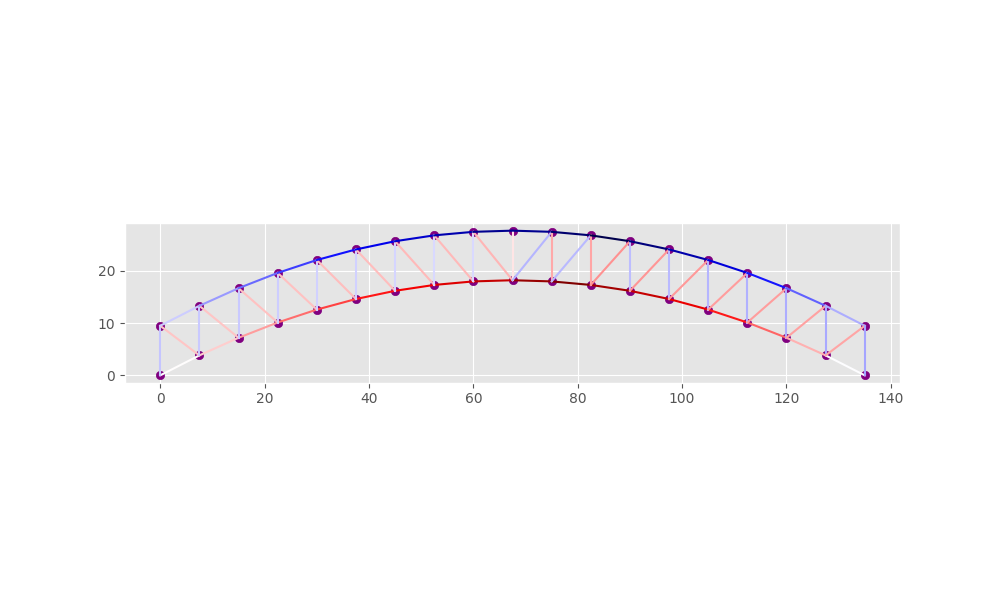
\includegraphics[width=\textwidth, trim=30 20 30 20, clip]{Fuerzas_reticulado_p5_pos12.png}
		\caption{Posición 12}
		\label{fig:p3_12}
	\end{subfigure}
	\caption{Diagrama de esfuerzos - carga de 240 kN para posiciones 9 a 12}
	\label{fig:esfuerzos_p3_c}
	
\end{figure}
\begin{figure}[H]\ContinuedFloat
	\centering
	
	% Fila 7
	\begin{subfigure}[b]{0.48\textwidth}
		\centering
		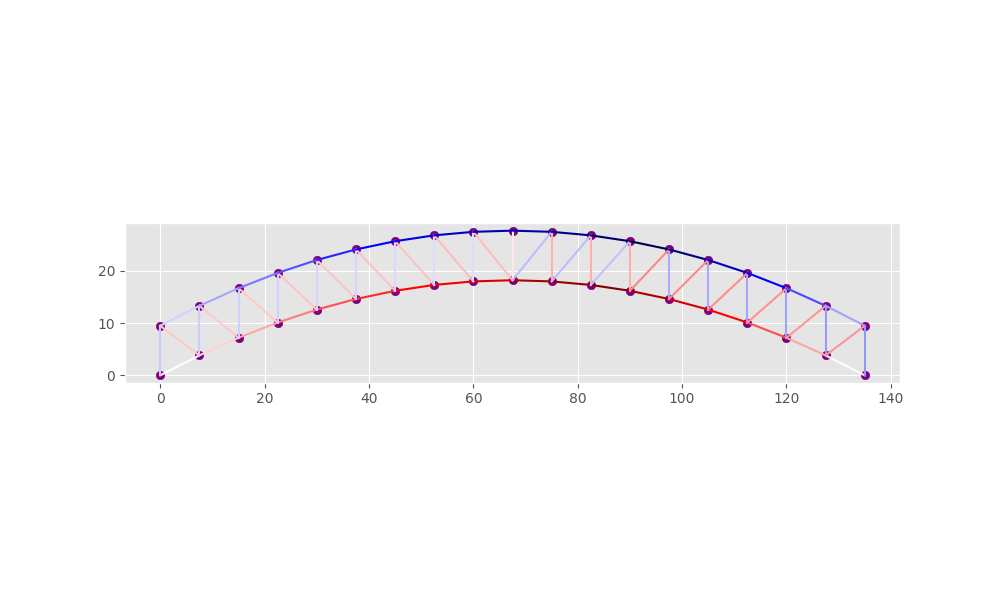
\includegraphics[width=\textwidth, trim=30 20 30 20, clip]{Fuerzas_reticulado_p5_pos13.png}
		\caption{Posición 13}
		\label{fig:p3_13}
	\end{subfigure}
	\hfill
	\begin{subfigure}[b]{0.48\textwidth}
		\centering
		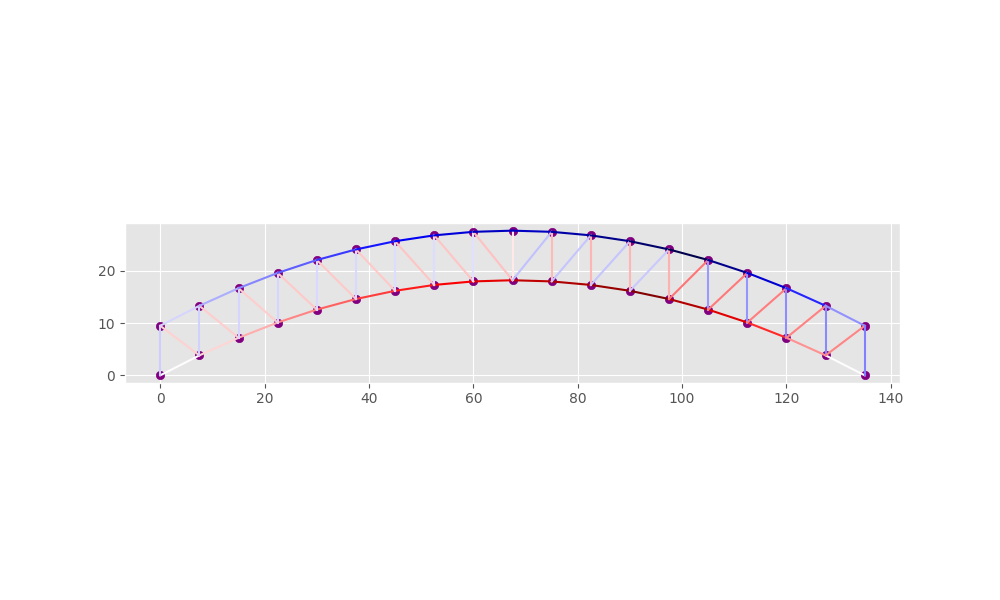
\includegraphics[width=\textwidth, trim=30 20 30 20, clip]{Fuerzas_reticulado_p5_pos14.png}
		\caption{Posición 14}
		\label{fig:p3_14}
	\end{subfigure}
	
	\vspace{3mm}
	
	% Fila 8
	\begin{subfigure}[b]{0.48\textwidth}
		\centering
		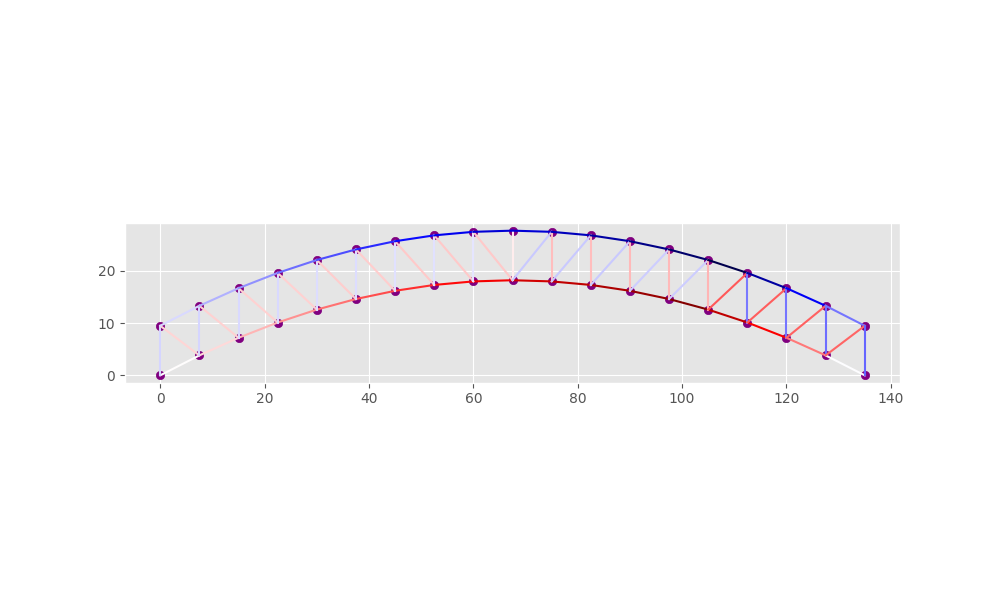
\includegraphics[width=\textwidth, trim=30 20 30 20, clip]{Fuerzas_reticulado_p5_pos15.png}
		\caption{Posición 15}
		\label{fig:p3_15}
	\end{subfigure}
	\hfill
	\begin{subfigure}[b]{0.48\textwidth}
		\centering
		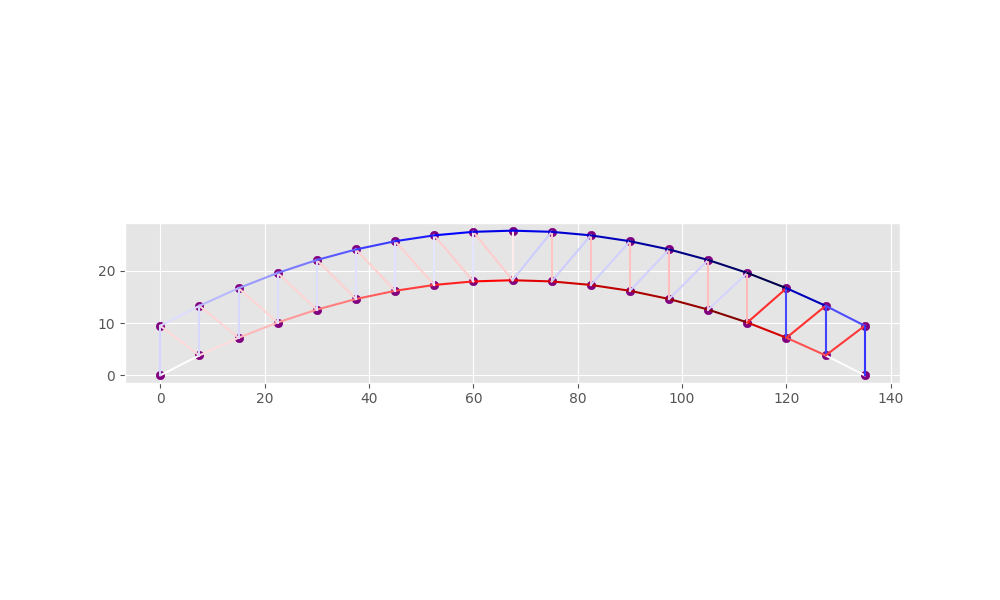
\includegraphics[width=\textwidth, trim=30 20 30 20, clip]{Fuerzas_reticulado_p5_pos16.png}
		\caption{Posición 16}
		\label{fig:p3_16}
	\end{subfigure}
	\caption{Diagrama de esfuerzos - carga de 240 kN para posiciones 13 a 16}
	\label{fig:esfuerzos_p3_d}
	
\end{figure}
\begin{figure}[H]\ContinuedFloat
	\centering
	
	% Fila 9
	
	\begin{subfigure}[b]{0.48\textwidth}
		\centering
		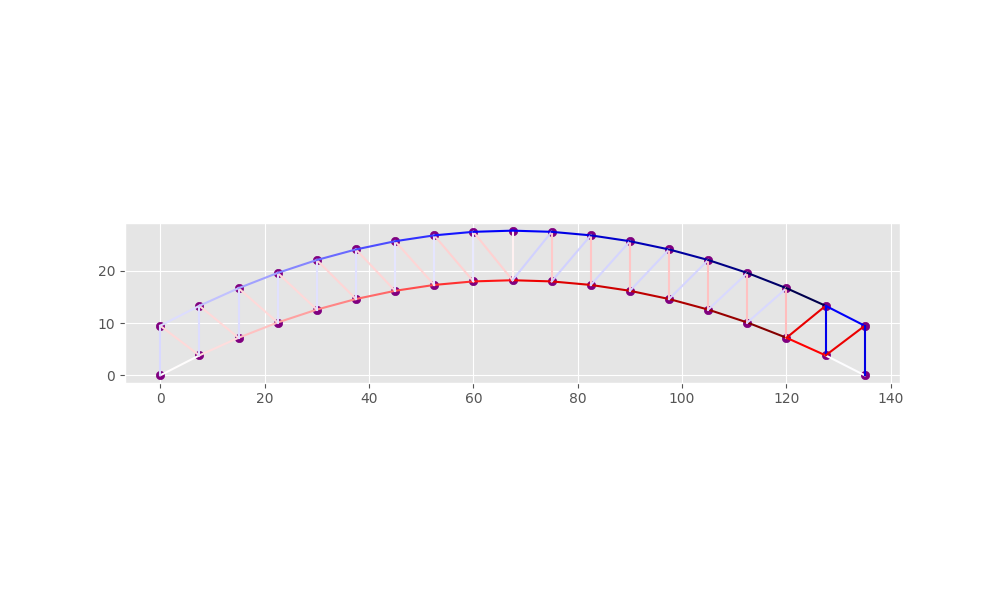
\includegraphics[width=\textwidth, trim=30 20 30 20, clip]{Fuerzas_reticulado_p5_pos17.png}
		\caption{Posición 17}
		\label{fig:p3_17}
	\end{subfigure}
	\hfill
	\begin{subfigure}[b]{0.48\textwidth}
		\centering
		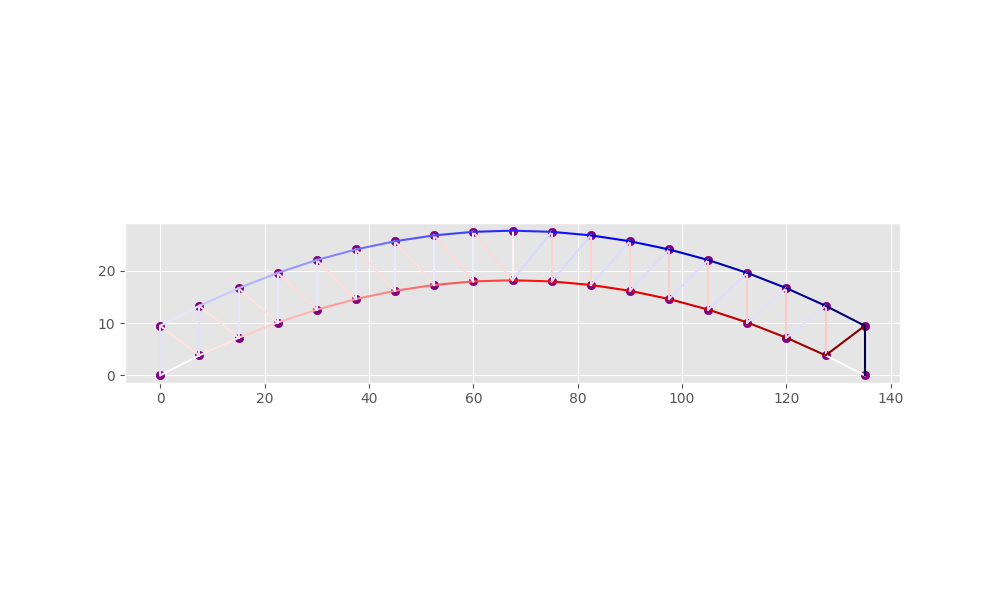
\includegraphics[width=\textwidth, trim=30 20 30 20, clip]{Fuerzas_reticulado_p5_pos18.png}
		\caption{Posición 18}
		\label{fig:p3_18}
	\end{subfigure}
	
	\vspace{3mm}
	
	%fila 10
	
	\begin{subfigure}[b]{0.48\textwidth}
		\centering
		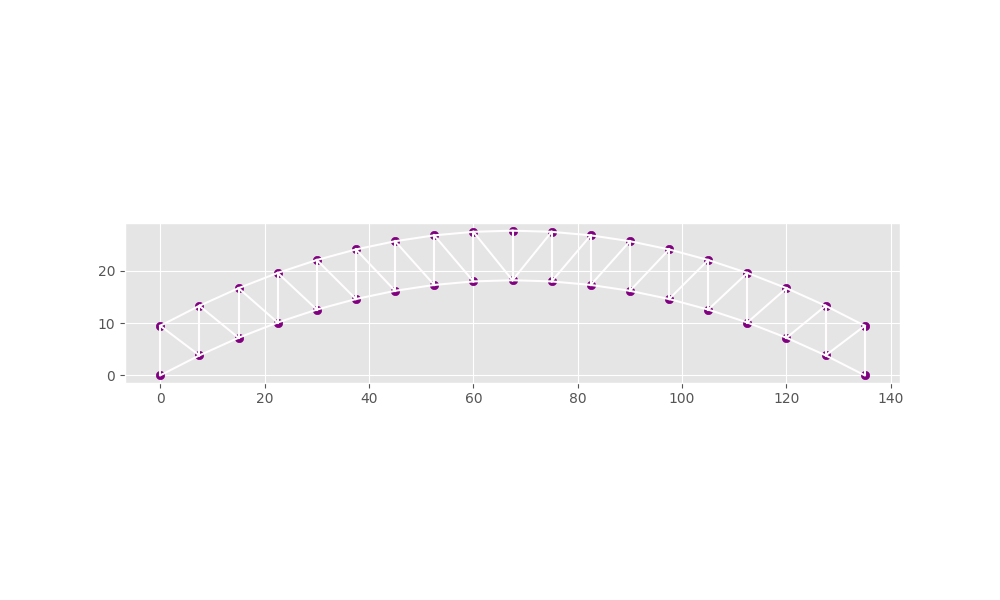
\includegraphics[width=\textwidth, trim=30 20 30 20, clip]{Fuerzas_reticulado_p5_pos19.png}
		\caption{Posición 19}
		\label{fig:p3_19}
	\end{subfigure}
	\caption{Diagrama de esfuerzos - carga de 240 kN para posiciones 17 a 19 }
	\label{fig:esfuerzos_p3_e}
	
\end{figure}
	
	\section{Análisis de Resultados}
	\subsection{Problema 1}
	La validez de los resultados obtenidos puede ser verificada mediante comprobaciones de equilibrio global: la suma vectorial de las fuerzas externas debe ser igual a la suma de las reacciones expresadas por \textbf{Rid}. Mediante la visualización por colores podemos identificar de forma intuitiva los elementos más solicitados de los cuales: tonos rojos indican tracción y tonos azules indican compresión, donde la intensidad del color se ve relacionada de manera proporcional a la magnitud del esfuerzo. El color blanco indica un esfuerzo nulo

	\subsection{Problema 2}
	Para este problema podemos ver que mantiene la misma lógica anterior con diferencia única la de incorporar el coseno director correspondiente al eje z. Los resultados son verificables bajo los mismos métodos comentados para el problema 1, es decir mediante equilibrio global en las tres direcciones coordenadas.
	
	\subsection{Problema 3}
	El perfil parabólico adoptado llega a una altura de 18,225 m en su punto máximo, la mitad de la distancia máxima, garantizando de esta forma el espacio suficiente solicitado para el flujo náutico. Adoptar una forma parabólica resulta particularmente ventajoso por su capacidad de distribuir los esfuerzos de forma gradual, como se puede apreciar en los respectivos diagramas de esfuerzo.
	
	Se puede observar que los elementos numerados como 0 y 17, correspondientes a los extremos de la pista vehicular, presentan un esfuerzo interno igual a 0 independiente de la posición en la que se encuentre la carga En los nodos extremos solo llegan dos elementos el tramo de la pista y el elemento perfectamente vertical, al ser el apoyo de A una rotula deslizante, no existe una componente horizontal la cual equilibrar, lo cual fuerza a que el esfuerzo de los tramos extremos sea nulo.
	
	Respecto a la seguridad de la estructura podemos afirmar que los elementos con estado mas críticos corresponden a los elementos \textbf{(8, 9, 41, 44, 46, 49)} debido a que entre todos tienen un FS $\geq$ 3
	el hecho de que todos los factores de seguridad sen considerablemente menores a 1, indica que el puente si cumple con absolutamente todas las restricciones de resistencia planteadas para todas las configuraciones analizadas de la carga móvil.
	\section{Conclusión}
	El desarrollo de la presente tarea dio la oportunidad para implementar de manera exitosa el método matricial de análisis de reticulados ya sea para casos 2D o 3D. Del trabajo realizado se pudo extrapolar las siguientes conclusiones:
	\begin{itemize}
		\item La formulación a modo matricial de cualquier estructura de reticulado isoestatica puede  automatizar el proceso de resolución de estas y facilitar el proceso de calculo estructural mediante programas computacionales
		\item El diseño parabólico del puente con parámetros obtenidos de las restricciones planteadas por las necesidades del sistema resultó en un sistema que cumple a la perfección con lo que se espera de este
	\end{itemize}
	
	\section{Declaración uso IA}
	Para la resolución de esta tarea se utilizo inteligencia artificial con los siguientes propósitos:
	\begin{itemize}
		\item Comprensión de conceptos relacionados al método matricial para reticulados
		\item Lista de comandos para redacción del informe en formato LaTeX
	\end{itemize}

	
	\section{Bibliografía}
	\begin{itemize}
		\item Matplotlib documentation — Matplotlib 3.10.9 documentation. (s. f.). \url{https://matplotlib.org/stable/}
		\item pyplot — Matplotlib 1.4.2 documentation. (s. f.). \url{https://matplotlib.org/1.4.2/api/pyplot_api.html#matplotlib.pyplot.plot}
		\item NumPy documentation — NumPy v2.4 Manual. (s. f.). \url{https://numpy.org/doc/stable/index.html}
		
	\end{itemize}
	
\end{document}